\documentclass[aps,prc,preprint,superscriptaddress,showpacs,showkeys]{revtex4-1}
\usepackage{graphicx}
\usepackage[usenames,dvipsnames,svgnames,table]{xcolor}


\begin{document}

\newcommand{\fm}{\mbox{fm}}
\newcommand{\MeV}{\mbox{MeV}}
\newcommand{\GeV}{\mbox{GeV}}

\title{{\Large Direct photon production at RHIC and LHC}}
\author{\large Vineet Kumar}
\author{\large Prashant Shukla}
\email{pshukla@barc.gov.in}
\affiliation{Nuclear Physics Division, Bhabha Atomic Research Center, Mumbai, India}
\affiliation{Homi Bhabha National Institute, Anushakti Nagar, Mumbai, India}
\date{\today}



\begin{abstract}

In this work, the photon spectrum measured in RHIC and LHC  
experiments at $\sqrt{s_{\rm NN}}$ = 0.2 and 2.76 TeV respectively has been 
analyzed in a hydrodynamical model. The data is compared with the calculations.
The data shows enhancement even after considering all the known sources of
direct photon production. Surprisingly enhancement factor is found to be 
more at RHIC energy than the LHC energy. 
\end{abstract}

\pacs{12.38.Mh, 24.85.+p, 25.75.-q}
\keywords{quark-gluon plasma, direct photon}

\maketitle

\section{Introduction} \label{Introduction}

  The ultra relativistic heavy ion collision experiments are performed 
with the aim to produce matter with very high energy density required to 
form quark gluon plasma (QGP). With this aim, Pb+Pb collision experiments 
at $\sqrt s = 17.6A$ GeV have been carried out at CERN SPS giving a 
variety of data on electromagnetic and hadronic observables
[For a review see \cite{ESKOLA}]. 
  The most interesting are the electromagnetic probes \cite{WA98}, 
which are sensitive to various stages of the evolution of the system and 
may contain the information about QGP formation. 
  A considerable amount of theoretical work has been done 
to dig out the information on QGP from these 
data [For review see~\cite{GALER,PEITZ}].

  To explain the data with hydrodynamical models, one assumes that QGP 
is formed with given initial conditions which then expands
hydrodynamically till it reaches the critical temperature $T_C$ for 
quark-hadron phase transition.
  In the idealized Maxwell construction, the temperature of the system 
is held fixed at $T=T_C$ until the hadronization is completed. 
Thus in turn one assume that the latent heat obtained by the phase 
transition is compensating the temperature drop due to cooling.
Such a picture has been widely used in literature when describing
the electromagnetic signals \cite{SRIVASTAVA}.
  This is a good approximation when the expansion time scales are far 
greater than the phase transition time scales as in the case of early 
universe. 
  For the case of relativistic heavy ion collisions, there have
been extensive studies of the space time evolution of 
QGP undergoing a first order phase transition by nucleation
\cite{CSER,SHUK,INHOMO,ZABPC}.
  As a result of rapid expansion of the system, a substantial amount of 
supercooling is expected and the dynamics of quark hadron phase 
transition becomes quite different in RHIC as compared to that 
in early universe \cite{INHOMO,AKM}. 
 When the hydrodynamical equations are coupled with nucleation rate 
equation \cite{INHOMO}, the QGP is shown to supercool to a temperature 
$T_S$ lower than $T_C$. The hadronization proceeds by thermal fluctuation
from this metastable QGP to stable hadron phase. The system 
reheats due to the release of latent heat and approaches to $T_C$ as 
the hadronization proceeds. Such a calculation is shown in Fig.~1.
This corresponds to an equilibrium situation where the latent heat 
generated is going into reheating the system. 

It is also possible that QGP supercools to a temperature,
the barrier between the metastable QGP and the stable hadron phase minima 
completely vanishes leading to a point of inflection at $T=T_S$ known as 
spinodal instability \cite{SPINO}. In this case, the rapidly quenched system 
leaves the region of metastability and enters the highly unstable spinodal 
region before a substantial amount of nucleation begins.
If it happens, then one can not define the phase transition rate by 
thermal fluctuation.

   The spinodal decomposition has also been suggested as a
possible mechanism of phase conversion for a rapidly expanding system of 
quarks and gluons \cite{SPINO,DUMHEP,DUMPRL}. This hadronization process
is much faster than the nucleation and is  
also referred as explosive decomposition \cite{DUMEXP}.
 The QGP breaks up into small droplets of plasma, which will form hadrons. 
 This occurs in a short time and the system may not be able to undergo 
further reequilibration and would freeze out at this point. 
  Such a picture has been presented in literature many times
and referred as 'a fast shock like hadronization' in 
Refs.~\cite{CSORGO} and a 'sudden hadronization scenario' in 
Ref.~\cite{RAFEL}.
  The signature of such a scenario will be very short life time 
\cite{CSERNAI} of the system measured through HBT data \cite{NA49,PHEN} 
and should combine with no mass shift observed in $\rho$ and $\phi$.

  When most of the QGP volume has been converted to hadrons, 
the already nucleated hadron bubbles would tend to join together and 
the QGP droplets will be trapped inside. At such a point, fluctuation 
theory is no more applicable. The system is highly unstable at this point 
and may simply breaks up into fragments: hadronic clusters and small 
droplets of plasma which then form the final state hadrons \cite{ZABPRC}. 

  As all these scenarios exist in the literature, it is worthwhile 
to see their manifestation in the measured photon spectrum 
which is the best probes of space time evolution of 
quark-gluon plasma (QGP) possibly produced in relativistic heavy-ion
collisions. Direct photon spectra have been measured by
the WA98 collaboration at the SPS~\cite{WA98}.

   In the present work, the contribution of thermal photons  
are calculated and compared with SPS data, assuming the QGP formation which 
expands and goes through supercooling.


\section{Hydrodynamic Model}

We consider that QGP is formed at some initial temperature $T_i$ and
initial time $\tau_i$ and starts cooling. The evolution of the system for each 
centrality of collision is governed by an isentropical cylindrical expansion with volume element
\begin{equation}
V(\tau) = \tau\,\pi\,(R + {1\over 2} a \, \tau^2 )^{2},
\end{equation}
 where a$_T$=0.1c$^2$ fm$^{-1}$ is the transverse acceleration \cite{Zhao:2011cv}.
 The initial transverse size, $R$ as a function of centrality is obtained as 
\begin{equation}
R(N_{\rm part}) = R_{0-5\%} \, \sqrt{N_{\rm part} \over (N_{\rm part})_{0-5\%} },
\label{RVsNPart}
\end{equation}
where $R_{0-5\%} = 0.96\,R_{\rm Pb}$; $R_{\rm Pb}$ being the radius of the Pb nucleus.

The evolution of entropy density for each centrality is obtained by entropy conservation 
condition $s(T)\,V(\tau)= s(T_0)\,V(\tau_0)$.
The equation of state obtained by Lattice QCD along with hadronic resonance gas \cite{Huovinen:2009yb} 
is used to obtain the temperature as a function of proper time $\tau$.
  The initial entropy density for each centrality is calculated using 
\begin{equation}
s(\tau_0) = s(\tau_0)|_{0-5\%} \left(\frac{dN/d\eta}{N_{\rm part}/2}\right)/\left(\frac{dN/d\eta}{N_{\rm part}/2}\right)_{0-5\%}.
\label{TempNpart}
\end{equation}
Measured values of $\left(\frac{dN/d\eta}{N_{\rm part}/2}\right)$ as a function of $N_{\rm part}$ 
\cite{Aamodt:2010cz,Chatrchyan:2011pb} are used in the calculations.

The initial entropy density $s(\tau_0)|_{0-5\%}$ for 0-5\% centrality is obtained as 
\begin{eqnarray}
s(\tau_0)|_{0-5\%}  = {a_{\rm m} \over V(\tau_0)|_{0-5\%}}   \left(\frac{dN}{d\eta}\right)_{0-5\%} . 
\label{TempVsMult}
\end{eqnarray}  
 Here $a_m$ (= 5 ) is a constant which relates the total entropy with the multiplicity. It is
obtained from hydrodynamic calculations \cite{Shuryak:1992wc}. 
Using $(dN/d\eta)_{0-5\%}$=1.5$\times$1600 obtained from the charge particle multiplicity measured in PbPb 
collisions \cite{Aamodt:2010cz,Chatrchyan:2011pb} at 2.76 TeV and with lattice
equation of state we obtain the initial temperature for the most central collisions 
as 0.492 GeV at time $\tau_0$ = 0.3 fm/c. To estimate the initial temperature $T_{0}$ in 
forward rapidity we use measured charged particle density $(dN/d\eta)$ in forward rapidity \cite{Abbas:2013bpa}. 
For ALICE rapidity coverage $[2.5\leq y \leq 4]$ the average temperature in most central 0-5\% collisions 
is found to be 0.434 GeV at time $\tau_0$ = 0.3 fm/c.

The (proper) time evolution of temperature is shown in Fig.~\ref{fig:TauVsTemp}(a) 
and that of QGP fraction in Fig.~\ref{fig:TauVsTemp}(b), in case of most central (0-5$\%$) collisions.
Here we compare the evolutions obtained with longitudinal and cylindrical expansions using 
both first order and lattice Equation of state (EOS). 
 For the first order EOS, $T_C$ = 0.170 GeV and the QGP fraction goes from 1 to 0 at this
temperature assuming a mixed phase of QGP and hadrons.
  The QGP fraction in case of lattice EOS governs number of degrees of freedom 
decided by entropy density. It is fixed to 1 above an entropy density 
corresponding to a 2-flavour QGP and fixed to zero below entropy density for a hot 
resonance gas. The freeze out temperature in all cases is $T_f=0.140$ GeV.  


\begin{figure}
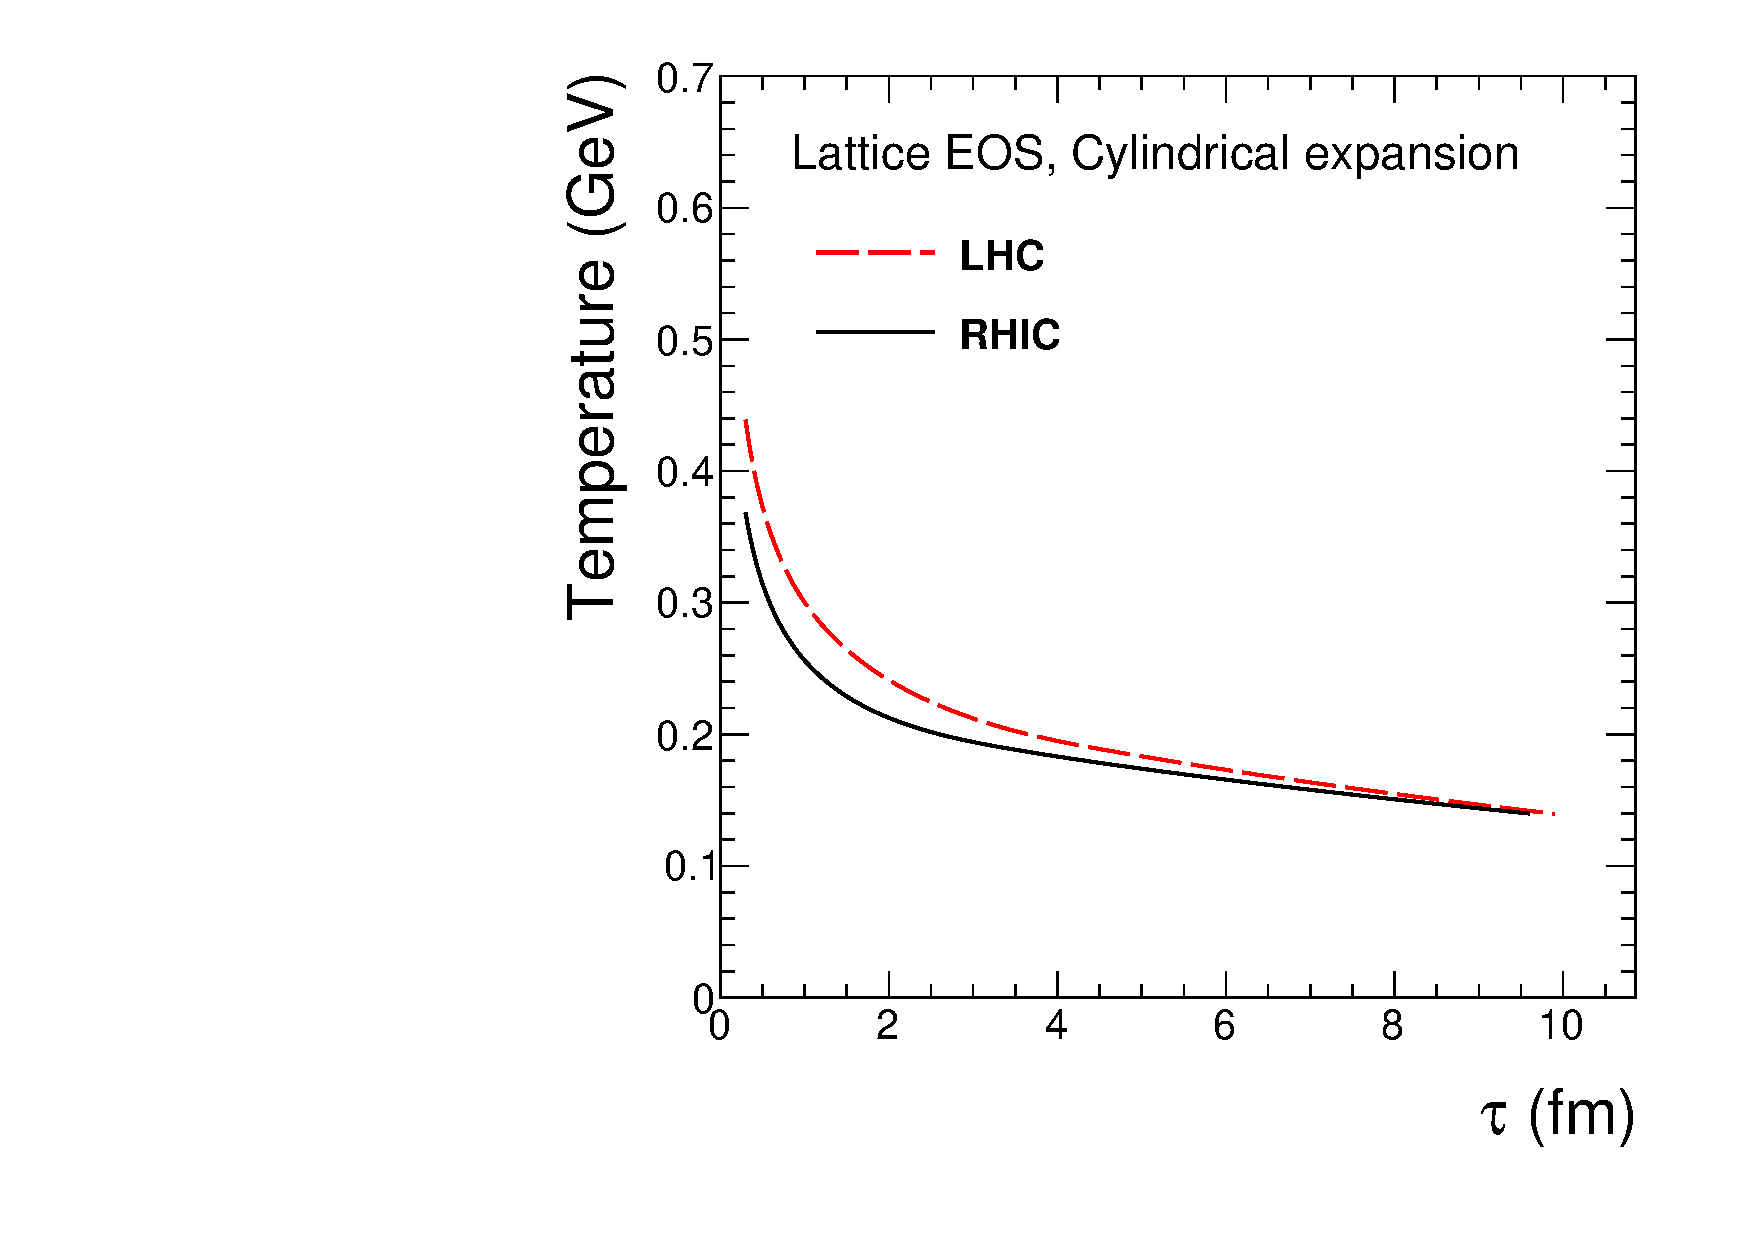
\includegraphics[width=0.49\textwidth]{Figures/Fig1a_TempVsTauLatt.pdf}
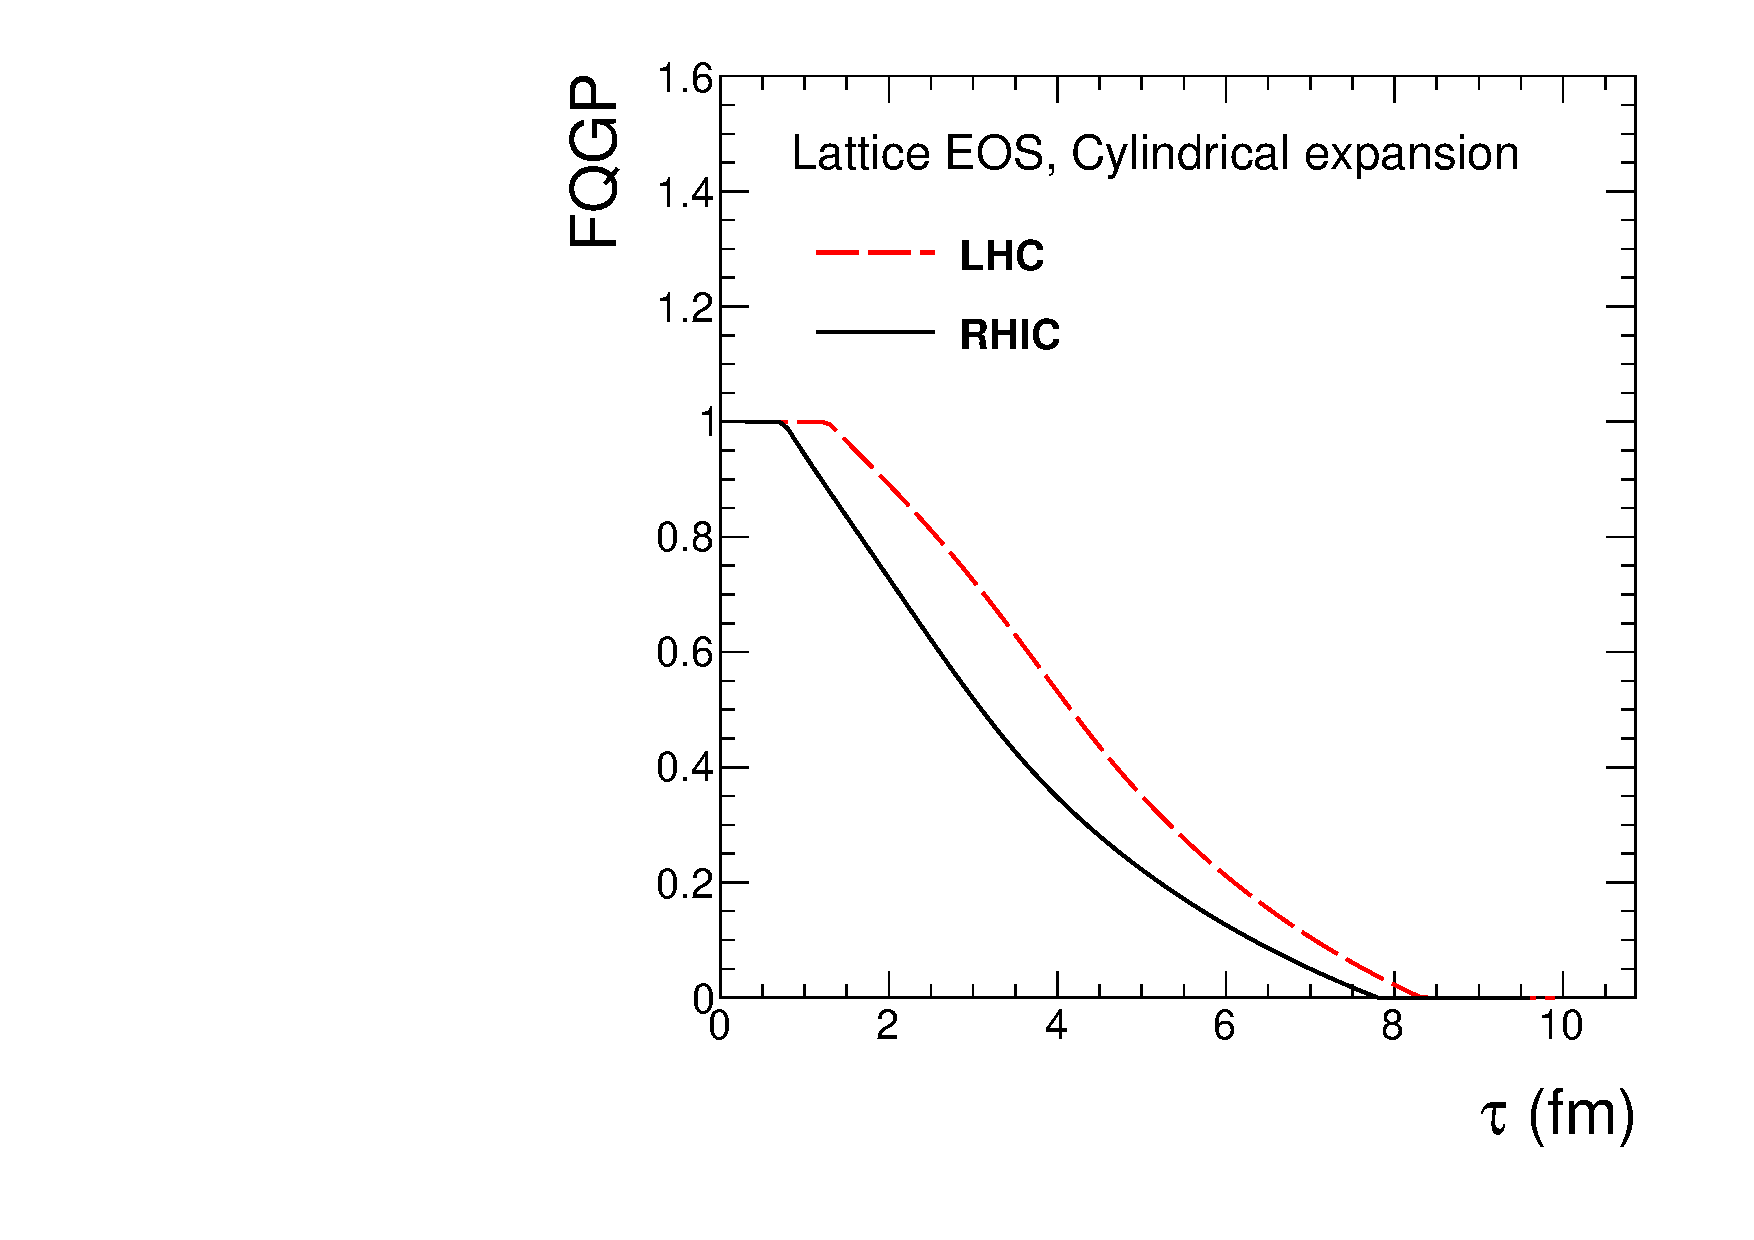
\includegraphics[width=0.49\textwidth]{Figures/Fig1b_FQGPVsTauLatt.pdf}
\caption{(Color online) (a) Temperature and (b) QGP fraction in the system as a function of proper 
time $\tau$ in case of the most central (0-5$\%$) collisions for longitudinal and cylindrical expansions 
using first order and lattice equation of state . }
\label{fig:TauVsTemp}
\end{figure}

%sTransverse expansion is not taken into account considering short 
%life time of the system. To get the equations of state it is assumed that 
%QGP is a massless 2 flavour parton gas and hadronic phase is a massless three 
%pion gas.

% When the QGP cools to the critical temperature $T_C$ we invoke 
%following four scenario for the calculations:

%(1) Idealized Maxwell construction (from $T_i$ to $T_f$.):
%    The temperature of the system is held fixed at $T=T_C$ until 
%    the hadronization is completed. Afterwards the hadron gas
%    cools to $T_f$ by hydrodyanmics.

%(2) Supercooling scenario (from $T_i$ to $T_f$.)
%   At $T_C$, hydrodynamical equations are coupled with nucleation 
%  rate equations \cite{IHOMO,SPINO}. The QGP 
%   supercools to a temperature $T_S$ lower than 
%  $T_C$ as shown in Fig.~1. The hadronization proceeds by 
%  thermal fluctuation from this metastable QGP phase to stable hadron phase. 
% The system reheats due to the release of latent heat and approaches to 
% $T_C$ as the hadronization proceeds. When hadronization is completed,  
% the hadron gas cools to $T_f$ by hydrodyanmics.

%(3) Spinodal decomposition followed by freeze out
%             (from $T_i$ to $T_S$.)
%   QGP supercools to a $T_S$ which is close to spinodal temperature
% \cite{SPINO}. The QGP breaks up into small droplets of plasma,
%which will form hadrons which then freezw out.


%(4) Fragmentation at 95 \% of hadronization followed by freeze out
%               (from $T_i$ to $T_P$.)
%  In the nucleation scenario (2) when 95 \% of the QGP volume has been 
%converted to hadrons, the system breaks up into fragments: hadronic clusters 
%and small droplets of plasma which then form the final state hadrons. 

%The total thermal photon/dilepton emission rate is given general by 
%the sum of corresponding rates $R_{\rm QGP}$ in the QGP and $R_{\rm hadron}$ 
%in the hadron regions integrated over space time volume 
%element $d^4x = \tau d\tau d\eta_f \pi R^2$ as
%\begin{eqnarray}\label{}
%R_I  &=& \int_{\tau_i}^{\tau_f} \int_{-l}^{l} 
%      \left[(1-h(\tau)) R_{\rm QGP}(T(\tau),\eta_f) 
%   + h(\tau)  R_{\rm hadron}(T(\tau),\eta_f) \right]\tau d\tau d\eta_f \pi R^2
%\end{eqnarray}
%Here $\eta_f$ is the fluid rapidity and $R$ is the size of colliding 
%nuclei given by $R=1.2\, A^{1/3}$. The $h(\tau)$ is the hadronic fraction
%at a time $\tau$.

% The temperature $T(\tau)$ and the hadronic fractions $h(\tau)$ are
%obtained using above two scenario. The temperature variation
%in the quark phase is governed by,
%\begin{eqnarray}\label{}
%T(\tau) = T_i \left({\tau_i \over \tau}\right)^{1/3}
%\end{eqnarray}

%While the temperature variation in the hadron phase is governed by,
%\begin{eqnarray}\label{}
%T(\tau) = T_h \left({\tau_h \over \tau}\right)^{1/3}
%\end{eqnarray}

% Assuming, Bjorken scaling, the experimentally observed rapidity 
%density $dN/dy$ can be related to the initial conditions by

%\begin{equation}
%dN/dy = \pi R_A^2 4 a_q T_i^3 \tau_i/3.6,
%\end{equation}
%where $a_q$ is the number of degrees of freedom in quark phase.
%The experimentally observed $dN/dy=1.5\, dN_{ch}/dy$ 





\section{The photon distribution}

  The production rate for hard thermal photons from an equilibrated 
QGP has been calculated in
perturbative thermal QCD applying the hard thermal loop (HTL)
resummation to account for medium effects. 


The {\em Compton scattering} and {\em $q\bar{q}$-annihilation} contribution
derived from the 1-loop HTL photon-polarization 
tensor~\cite{KAPUSTA_1991,BAIER_1991,TRAXLER_1995} is given by
%
\begin{equation} 
 E\,\frac{dN}{d^4x\,d^3p} \, =  {5\over 18 \pi^2}\,\alpha \alpha_s 
       \ln \left(\frac{0.23\,E}{\alpha_s\,T}\right)
            \,T^2\,e^{-E/T},
\label{1-loop}
\end{equation}
%
The contributions from {\em bremsstrahlung}, 
and {\em $q\bar{q}$-annihilation with an additional scattering in the medium},
obtained from the 2-loop HTL photon-polarization
tensor~\cite{AURENCHE_1998,THOMA} are given by
%
\begin{equation} 
   E\,\frac{dN}{d^4x\,d^3p} \, = 
        0.0219\,\alpha \alpha_s
        \,T^2\,e^{-E/T},
\label{bremss}
\end{equation}
%

%
\begin{equation} 
      E\,\frac{dN}{d^4x\,d^3p} \, =  
        0.0105\,\alpha \alpha_s
        \,E\,T\,e^{-E/T},
\label{qqbar-aws}
\end{equation}
%

All three rates are listed for a two-flavored
($N_f = 2$) QGP. Here $\alpha=1/137$ and the strong coupling constant is 
$\alpha_s= 6\pi/((33-2N_f) \ln(8T/T_C))$ \cite{KARSCH}.
The rates~(\ref{bremss}) and~(\ref{qqbar-aws}) were 
{\em erroneously} multiplied 
by a factor of 4 \cite{AURENCHE_1998}, 
we take the rates in correct form \cite{THOMA}.

Here $E=P_T \cosh(y-\eta_f)$ where $y$ is the rapidity in the center
of mass frame and $\eta_f$ is the fluid rapidity.

 The thermal photon production in an equilibrated hadron phase
is determined by considering various meson interactions
$\pi \pi \rightarrow \rho \gamma$, $\pi \rho \rightarrow \pi
\gamma$, $\omega \rightarrow \pi \gamma$ and $\rho
\rightarrow \pi \pi \gamma$~\cite{KAPUSTA_1991,NADEAU_1992}.  By considering
additionally the $\pi \rho \rightarrow a_1 \rightarrow \pi \gamma$ reaction, a
strong enhancement of the rate was observed~\cite{XIONG_1992}. 
 The numerical results of a detailed study of these dacays has been
fitted by analytical expression as a function of temperature and photon
energy as reported in Ref.~\cite{THOMA} given as
%
\begin{equation} 
        E\,\frac{dN}{d^4x\,d^3p} \, = 
        4.8\,T^{2.15}\,e^{-1/(1.35\,T\,E)^{0.77}}\,e^{-E/T},
\label{Markus_suggestion}
\end{equation} 
%
where photon energy~$E$ and temperature~$T$ are to be given in GeV to obtain the
rate in units of $\fm^{-4}\GeV^{-2}$. 

{\bf Prompt Photons}. 
 Dumitru et al. \cite{DUMI} estimate the contribution of prompt photons 
which employs the pQCD with inclusion of the effect of intrinsic 
transverse momentum of the partons. Their results for Pb+Pb collision
$\sqrt{s} = 17.4 A$GeV for $<K_T^2>=1.8$ GeV$^2$ including additional 
broadening from nuclear effects can be parameterized as 
\begin{equation}\label{promp}
 E \frac{d^3 N}{d^3 p} = \exp(a + bP_T + cP_T^2 + dP_T^3)
\end{equation}
where $a=-4.1506$, $b=-1.9845$, $c=0.0744$, and 
$d=-0.0383$.

 In the work of Gallmeister~\cite{GALLMEISTER} hard photon 
 yield is generated by the event generator PYTHIA and are
parameterized same as Eq.~(\ref{promp}) with the coefficients
$a=-5.9883$, $b=2.0934$, $c=-1.6015$ and $d=0.1432$.
 The WA98 direct photon data analysis of Gallmeister et al.\ obtained in 
a model describing a {\em spherically} symmetric 
expansion~\cite{GALLMEISTER}.

 It is also possible to reproduce the WA98 direct photon data analysis of
Srivastava et al.~\cite{SRIVASTAVA}, which does not necessitate prompt
photons but instead initial conditions that are rather extreme for SPS, i.e.\ a
very small thermalization time of $\tau_0 = 0.2\;\fm$ and a very high initial
temperature of $T_0 = 335\;\MeV$. 
The effective degrees of freedom in the hadron gas has been increased
from the actual value of $g_h = 3$ to an effective one of $g_h =8$ in order 
to achieve the fit in the HHG thermal photon spectrum. This reduces
the life of mixed phase and hence reducing the contribution from 
hadron phase.


For {\em typical} parameters 
%
$\tau_i = 0.8\;\fm$, $T_i = 210\;\MeV$, $T_c = 160\;\MeV$, $T_f = 140\;\MeV$, 
%
nucleon number $A=208$ (corresponding to Pb + Pb collisions)
we have obtained the photon spectrum.










\section{The dilepton distribution}

 The dilepton emission rate in the quark sector considering the 
processes ($q \bar q \rightarrow e^- e^+$)
is given \cite{KAJA,VOGT} by 

\begin{eqnarray}\label{}
 {dN \over d^4x d^2p_T dy dM^2}
&=& \frac{3}{(2\pi)^5} M^2 \sigma(M^2)
        \exp\left(-\frac{E}{T}\right), \nonumber \\
&=& \frac{\alpha^2}{8\pi^4} \left(\sum e_q^2\right) 
        \exp\left(-\frac{E}{T}\right).
\end{eqnarray}
Here, $\sigma(M^2)=4\pi\alpha^2/3M^2$ and $F_q = \sum e_q^2 = 5/9$.

The dilepton emission rate from hadron phase is given by
\begin{eqnarray}\label{}
\frac{dN}{d^4x d^2p_T dy dM^2} = \frac{\alpha^2}{8\pi^4}\, F_h \,
 \exp(-{E\over T}),
\end{eqnarray}
For the hadrons, if we assume 
$\pi\pi \rightarrow \rho \rightarrow l^+l^-$ is the dominant channel, 
\begin{eqnarray}\label{}
F_h = \frac{1}{12} \frac{m_\rho^4}{(m_\rho^2-M^2)^2 + m_\rho^2 \Gamma_\rho^2}
\end{eqnarray}
The parameters used are $m_\rho$=768 MeV, $\Gamma$=151 MeV. The detail
form factors can be obtained from Ref.~\cite{GALE}

We get, the $p_T$ distribution as
\begin{eqnarray}\label{}
\frac{dN}{d^4x dy dM^2 p_T dp_T } = \frac{\alpha^2}{4\pi^3}  F \,
   \exp\left(-\frac{ \sqrt{M^2 + p_T^2} cosh (y-\eta)}{T}\right)
\end{eqnarray}

and the invariant mass distribution 
\begin{eqnarray}\label{}
\frac{dN}{d^4x dy dM} = \frac{\alpha^2}{2\pi^3} F \, M^3 \,
\left({1\over x^2} + {1\over x}\right) \exp(-x),
\end{eqnarray}
where

\begin{eqnarray}\label{}
x=\frac{ M \cosh (y-\eta)}{T}.
\end{eqnarray}

Here $M$, $p_T$ and $y$ are the mass, transverse momentum,
and  rapidity of the lepton pair and $\eta$ is the rapidity
of the fluid with temperature $T$.

\section{Results and discussions}

  The total thermal photon emission rate is given by the sum of 
corresponding rates in the QGP and in the hadron regions integrated 
over space time volume obtained from above four scenario. The photon 
production rates are taken from the parameterized forms of Ref.~\cite{THOMA}.
 The contribution of prompt photons has been obtained by the PYTHIA
calculations \cite{GALLMEISTER}, while photons from the decay of hadrons
after freeze-out are already subtracted in the experimental analysis.

   Figure~2 demonstrates how the thermal photons contributions due to 
different evolutions compare with SPS data. 
From this figure, scenario (3) seems the most appropriate evolution scenario. 
 It must be noted that these calculations depend on the initial conditions, 
equation of state, photon rates and hydrodynamical expansion but, would 
certainly be helpful to understand the various evolution scenarios and their 
manifestation in photon spectrum.


\begin{thebibliography}{00}

\bibitem{ESKOLA} K. J. Eskola, {\it High Energy Nuclear Collisions}, 
  Plenary talk given at Int. Europhysics conference on High Energy Physics 
  (EPS-HEP99), Tampere, Finland, July 15-21, 1999, 
  Preprint: hep-ph/9911350 (1999).
  
\bibitem{WA98} WA98 Collab., M.M.\ Aggarwal et al., 
            Phys. Rev. Lett. 85, 3598 (2000); nucl-ex/0006007 (2000).






\bibitem{CERES} B. Lenkeit for CERES Coll., 
        Nucl. Phys. {\bf A654}, 627c (1999); nucl-ex/9910015.  
  
\bibitem{GALER} C. Gale, in {Quark Gluon Plasma 3}, World Scientific,
         Singapore, 2003. 
         
\bibitem{PEITZ} For recent review,  T. Peitzman, nucl-ex/0201003 (2002).

\bibitem{SRIVASTAVA} D.K.\ Srivastava and B.\ Sinha, nucl-th/0006018 (2000).

\bibitem{CSER} L.P. Csernai and J.I. Kapusta, Phys. Rev. Lett. {\bf 69},
               737 (1992).

\bibitem{SHUK} P. Shukla, S.K. Gupta, and A.K. Mohanty,
         Phys. Rev. C{\bf 59}, 914 (1999); {\it ibid} {\bf 62}, 39901 (2000).

\bibitem{INHOMO} P. Shukla, A.K. Mohanty, S. K. Gupta, and M. Gleiser,
              Phys. Rev. C{\bf 62}, 054904 (2000).

\bibitem{ZABPRC} E.E. Zabrodin, L.V. Bravina, H. Stocker, and W. Griener,
         Phys. Rev. C{\bf 59}, 894 (1999).


\bibitem{Zhao:2011cv} 
  X.~Zhao and R.~Rapp,
  ``Medium Modifications and Production of Charmonia at LHC,''
  Nucl.\ Phys.\ A {\bf 859}, 114 (2011).
  %[arXiv:1102.2194 [hep-ph]].

\bibitem{Huovinen:2009yb} 
  P.~Huovinen and P.~Petreczky,
  ``QCD Equation of State and Hadron Resonance Gas,''
  Nucl.\ Phys.\ A {\bf 837}, 26 (2010).
  %[arXiv:0912.2541 [hep-ph]].


\bibitem{Aamodt:2010cz} 
  K.~Aamodt {\it et al.}  [ALICE Collaboration],
  ``Centrality dependence of the charged-particle multiplicity density at mid-rapidity in Pb-Pb collisions at $\sqrt{s_{NN}}=2.76$ TeV,''
  Phys.\ Rev.\ Lett.\  {\bf 106}, 032301 (2011).
  %[arXiv:1012.1657 [nucl-ex]].
  

\bibitem{Chatrchyan:2011pb} 
  S.~Chatrchyan {\it et al.}  [CMS Collaboration],
  ``Dependence on pseudorapidity and centrality of charged hadron production in PbPb collisions at a nucleon-nucleon 
  centre-of-mass energy of 2.76 TeV,''
  JHEP {\bf 1108}, 141 (2011).
  %[arXiv:1107.4800 [nucl-ex]].

\bibitem{Shuryak:1992wc} 
  E.~V.~Shuryak,
  ``Two stage equilibration in high-energy heavy ion collisions,''
  Phys.\ Rev.\ Lett.\  {\bf 68}, 3270 (1992).
  
\bibitem{Abbas:2013bpa} 
  E.~Abbas {\it et al.}  [ALICE Collaboration],
  ``Centrality dependence of the pseudorapidity density distribution for charged particles 
  in Pb-Pb collisions at $\sqrt{s_{\rm NN}}$ = 2.76 TeV,''
  Phys.\ Lett.\ B {\bf 726}, 610 (2013).
  %[arXiv:1304.0347 [nucl-ex]].


\bibitem{AKM} A.K. Mohanty, P. Shukla and M. Gleiser,
              Phys. Rev. C{\bf 65}, 034908 (2002).
              
\bibitem{SPINO} P. Shukla and A. K. Mohanty, Phys. Rev. C{\bf 64},
        054910 (2001).              

\bibitem{DUMHEP} O. Scavenius, A. Dumitru, E.S. Fraga, J.T. Lenaghan,
         A.D. Jackson, Phys. Rev. D{\bf 63}, 116003 (2001).

\bibitem{DUMPRL} O. Scavenius, A. Dumitru,
         Phys. Rev. Lett. {\bf 83}, 4697 (1999).
         
\bibitem{DUMEXP} O. Scavenius, A. Dumitru, A.D. Jackson, 
          hep-ph/0103219.
          
\bibitem{CSORGO} T. Csorgo, L.P. Csernai, Phys. Lett {\bf B333}, 494 (1994);
       L.P. Csernai, I.N. Mishustin, Phys. Rev. Lett. {\bf 74}, 5005 (1995).
       
\bibitem{RAFEL} J. Rafelski and J. Letessier, Phys. Rev. Lett. {\bf 85},
                  4695 (2000).

\bibitem{CSERNAI} L.P. Csernai, M.I. Gorenstein, L.L. jenkovszky, 
                        I. Lovas and V.K. Magas, hep-ph/0210297.

\bibitem{NA49HBT} HBT

\bibitem{PHEN} PHENIX Collaboration, K. Adcox et. al., 
                    nucl-ex/0109003.

\bibitem{KAPUSTA_1991} J.\ Kapusta, P.\ Lichard, and D.\ Seibert, 
   Phys.\ Rev.\ {\bf D44}, 2774 (1991); {\bf D47}, 4171 (1993). 

\bibitem{BAIER_1991} R.\ Baier, H.\ Nakkagawa, A.\ Ni\'{e}gawa, and
K.\ Redlich, Z.\ Phys.\ {\bf C53}, 433 (1992).

\bibitem{TRAXLER_1995} C.T.\ Traxler, H.\ Vija, and M.H.\ Thoma,
Phys.\ Lett.\ {\bf B346}, 329 (1995).
  
\bibitem{AURENCHE_1998} P.\ Aurenche, F.\ Gelis, R.\ Kobes, and H.\ Zaraket,
  Phys.\ Rev.\ {\bf D58}, 085003 (1998); \mbox{hep-ph/9804224}. 

\bibitem{THOMA} F. D. Steffen and M. H. Thoma, Phys. Lett. B510, 
                  1998 (2001).
                  
\bibitem{KARSCH} F. Karsch, Z. Phys. C{\bf 38}, 147 (1988).
  
\bibitem{NADEAU_1992} H.\ Nadeau, J.\ Kapusta, and P.\ Lichard,
Phys.\ Rev.\ {\bf C45}, 3034 (1992); {\bf C47} 2426 (1993).

\bibitem{XIONG_1992} L.\ Xiong, E.\ Shuryak, and G.E.\ Brown, Phys.\
Rev.\ {\bf D46}, 3798 (1992).

\bibitem{DUMI} A. Dumitru, L. Frankfurt, L. Geland, H. Stocker, and
               M. Strikeman, Phys. Rev. C{\bf 64}, 054909 (2001).

\bibitem{GALLMEISTER} K.\ Gallmeister, B.\ K\"ampfer, and O.P.\ Pavlenko, 
            Phys. rev. C{\bf 62}, 057901 (2000); hep-ph/0006134 (2000).

\bibitem{SRIVASTAVA_SINHA_1999} D.K.\ Srivastava and B.C.\ Sinha,
             Eur.\ Phys.\ J.\ {\bf C12}, 109 (2000).

\bibitem{KAJA} K. Kajantie, M. Kataja, L. McLerran, and P. V. Ruuskanen,
               Phys. Rev. D{\bf 34}, 811 (1986).

\bibitem{VOGT} R. Vogt, B. V. Jacak, P. L. McGaughey, P. V. Ruuskanen,
          Phys. Rev. D {\bf 49}, 3345 (1994).
          
\bibitem{GALE} C. Gale and P. Lichard, Phys. Rev. D{\bf 49}, 3338 (1994);
               C. Song, C.M. Ko, and C. Gale, {\it ibit} 50 R 1827 (1994).
               
\bibitem{CUTS} J. SOllfrank, P. Huovinen, M. Kataja, P.V. Ruuskanen,
             M. Prakash and R. Venugopalan, 
             Phys. Rev. C{\bf 55}, 392 (1997).

\end{thebibliography}

\end{document}




